%Needs Package: 
%\usepackage{bm}
%\usepackage{multicol}
\section{LTI-Systeme}
\begin{minipage}{0.5\textwidth}

    \subsection*{Linearität und Zeitinvarianz}
    \begin{itemize}
        \item $\mathcal{T}[x_1(t) + x_2(t)] = y_1(t) + y_2(t)$
        \item $\mathcal{T}[k_a \cdot x(t)] = k_a \cdot y(t)$
        \item $\mathcal{T}[x(t-t_0) = y(t-t_0)]$
    \end{itemize}

    \subsection{Beschreibung von LTI Systemen}

    \subsubsection{Impulsantwort}
    Systemreaktion auf $\delta(t)$.

    $ y(t) = \mathcal{T}[x(t)]
        = \int \limits _{-\infty} ^{\infty} x(\tau) \cdot h(t-\tau)d\tau
        = x(t) * h(t)$

    \subsubsection{Frequenzantwort}
    Fouriertransformierte Impulsantwort.
    \\ Auch Übertragungsfunktion genannt.

    $$ Y(\omega) = X(\omega) \cdot H(\omega) = X(\omega) \cdot G(j\omega)$$

    \subsubsection{Berechnung des Ausgangssignals}
    1. Integraltransformation:
    \newline $X(\omega) = \mathcal{F}[x(t)] {\; \big / \;}
        X(s) = \mathscr{L}[x(t)]$ \\
    2. Berechnung in Bild / Frequenz:
    \newline $Y(\omega) = X(\omega) \cdot H(\omega)  {\; \big / \;}
        Y(s) = X(s) \cdot G(s)$ \\
    3. Rücktransformation:
    \newline $y(t) = \mathcal{F}^{-1}[Y(\omega)] = \mathscr{L}^{-1}[Y(s)]$

\end{minipage}%
\begin{minipage}{0.6\textwidth}


    \subsection{Bezeichnungen}
    Übertragungsfunktion: $H(\omega) = G(j\omega) =|H(\omega)| \cdot e^{j\varphi_H(\omega)}$ \\
    {\tiny auch: Frequenzgang}\\
    Amplitudengang: $|H(\omega)|$ \\
    Phasengang: $\varphi_H(\omega)$ \\

    \subsubsection{Filtereigenschaften}
    $Y(\omega) = X(\omega) \cdot H(\omega)$ \\
    $|Y(\omega)| = |X(\omega)| \cdot |H(\omega)|$ \\
    $\varphi_y(\omega) = \varphi_x(\omega) + \varphi_H(\varphi)$

    \subsection{BIBO-Stabilität \tiny {Bound-Input-Bound-Output}}

    Systemantwort Begrenzt, wenn Eingangssignal Begrenzt
    \newline $\Rightarrow$ Konvergenzhalbebene Übertragungsfunktion enthält Imaginär-Achse
    \newline $\Rightarrow$ Alle Polstellen Übertragungsfunktion links von "$j$-Achse"
    \begin{center}
        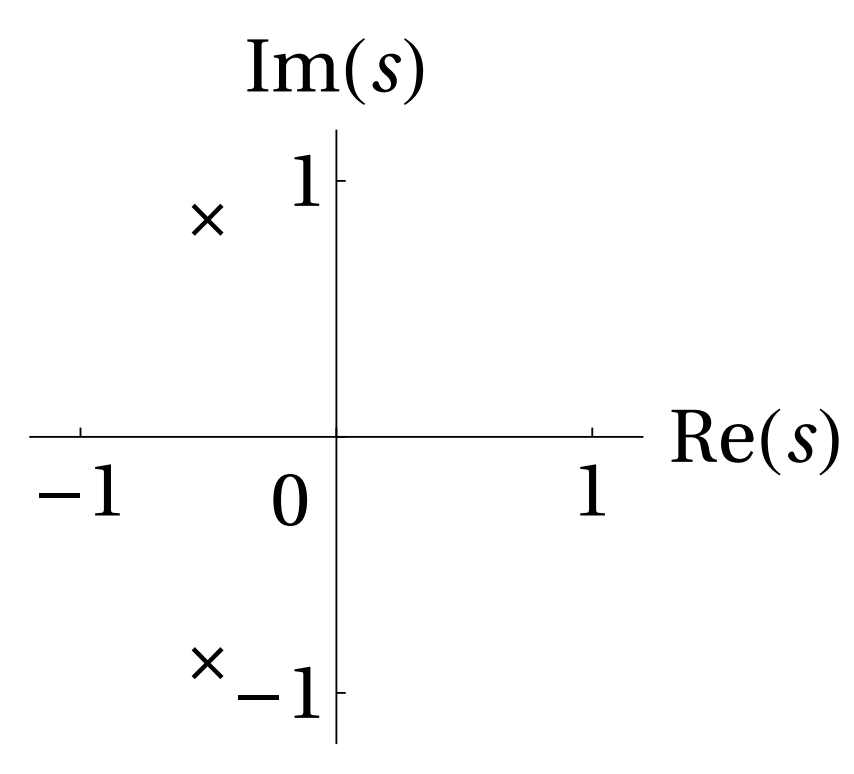
\includegraphics[width = 4cm]{include/Integraltransformationen/img/BiBo.png}
    \end{center}

\end{minipage}%
